% \iffalse meta-comment
% \preamble
% 
% Copyright (C) 2014 by Ben Reish
% -----------------------------------
%
% This file may be distributed and/or modified under the
% conditions of the LaTeX Project Public License, either version 1.3
% of this license or (at your option) any later version.
% The latest version of this license is in:
%
% http://www.latex-project.org/lppl.txt
%
% and version 1.3 or later is part of all distributions of LaTeX
% version 1999/12/01 or later.
% 
% \endpreamble
% \fi
%
% \iffalse
%<package>\NeedsTeXFormat{LaTeX2e}[1999/12/01]
%<package>\ProvidesPackage{blox}%
%<package>[2014/08/20 v2.5 Just an English translation of schemabloc]
%
%<*batchfile>
\begingroup
%%
%% Copyright (C) 2014 by Ben Reish
%%
%% This file may be distributed and/or modified under the
%% conditions of the LaTeX Project Public License, either
%% version 1.3 of this license or (at your option) any later
%% version. The latest version of this license is in:
%%
%% http://www.latex-project.org/lppl.txt
%%
%% and version 1.3 or later is part of all distributions of
%% LaTeX version 1999/12/01 or later.
%%
\input docstrip.tex
\keepsilent
\usedir{tex/latex/blox}
\preamble
This is a generated file.
Copyright (C) 2014 by Ben Reish
This file may be distributed and/or modified under the
conditions of the LaTeX Project Public License, either
version 1.3 of this license or (at your option) any later
version. The latest version of this license is in:
http://www.latex-project.org/lppl.txt
and version 1.3 or later is part of all distributions of
LaTeX version 1999/12/01 or later.
\endpreamble
\askforoverwritefalse
\generate{\file{blox.sty}{\from{blox.dtx}{package}}}
\Msg{*********************************************************}
\Msg{*}
\Msg{* To finish the installation you have to move the}
\Msg{* following file into a directory searched by TeX:}
\Msg{*}
\Msg{* \space\space blox.sty}
\Msg{*}
\Msg{* To produce the documentation run the file blox.dtx}
\Msg{* through LaTeX.}
\Msg{*}
\Msg{* Happy TeXing!}
\Msg{*********************************************************}
\endgroup
%</batchfile>
%<*driver>
\documentclass{ltxdoc}
\usepackage{blox}
\usepackage[colorlinks=true,urlcolor=blue,linkcolor=black,%
	citecolor=orange,pdfborder={0 0 0},%pdfpagemode=FullScreen,
	pdfdisplaydoctitle=true%
	]{hyperref}
\usepackage{fancyvrb}
\EnableCrossrefs
\CodelineIndex
\RecordChanges
\begin{document}
\DocInput{blox.dtx}
\end{document}
%</driver>
% \fi
%
% \CheckSum{261}
%
% \CharacterTable
% {Upper-case \A\B\C\D\E\F\G\H\I\J\K\L\M\N\O\P\Q\R\S\T\U\V\W\X\Y\Z
% Lower-case \a\b\c\d\e\f\g\h\i\j\k\l\m\n\o\p\q\r\s\t\u\v\w\x\y\z
% Digits \0\1\2\3\4\5\6\7\8\9
% Exclamation \! Double quote \" Hash (number) \#
% Dollar \$ Percent \% Ampersand \&
% Acute accent \' Left paren \( Right paren \)
% Asterisk \* Plus \+ Comma \,
% Minus \- Point \. Solidus \/
% Colon \: Semicolon \; Less than \<
% Equals \= Greater than \> Question mark \?
% Commercial at \@ Left bracket \[ Backslash \\
% Right bracket \] Circumflex \^ Underscore \_
% Grave accent \` Left brace \{ Vertical bar \|
% Right brace \} Tilde \~}
%
%
% \changes{v1.0}{2014/01/01}{Initial version}
% \changes{v2.0}{2014/08/01}{Fixed the chain mechanism to work with my implementation of tikz}
%
% \newcommand{\blox}{\textsf{blox}}
% \newcommand{\stikz}{\textsf{tikz}}
% \changes{v2.5}{2014/08/20}{Changed the name to \blox\ instead of \textsf{bloX} at CTAN's suggestion.}
%
% \newcommand{\verbatimfont}[1]{\renewcommand{\MacroFont}{\ttfamily#1}}
% \newcommand{\vrbfnt}{\verbatimfont{\fontsize{6pt}{8pt}\selectfont}}
%
% \GetFileInfo{blox.sty}
%
% \DoNotIndex{\#,\$,\%,\&,\@,\\,\{,\},\^,\_,\~,\ ,\@ne,\advance,\begingroup,\catcode,\closein,\closeout,\day,\def,\edef,\else,\empty,\endgroup,\newcommand,\draw,\newtoks,\ProvidesPackage,\RequirePackage,\node,\let,\global,\foreach}
%
% \title{The \textsf{blox} package\thanks{This document
% corresponds to \textsf{blox}~\fileversion,
% dated \filedate.}}
% \author{Ben Reish \\ \texttt{ben.reish@alumni.oc.edu}}
%
% 
%
% \maketitle
%
% \begin{abstract}
% The \textsf{blox} package is an English translation of the French \textsf{schemabloc} package for making block diagrams in \LaTeX2e.  Also, I fixed the chain feature to auto-create a linear linked chain of blocks from a list which did not work on my implementation of \textsf{tikz} and \textsf{schemabloc}.  
% \end{abstract}
%
% \section{Introduction}
%
% Have you ever needed to make a block diagram for a control system like Fig. \ref{fig:simpdia}?  Or, maybe to explain an algorithm?  The \blox\ package is an option to meet this need.  It allows for the use of most of \textsf{tikz}'s personalization capability for the blocks themselves and the lines.  But, the defaults look pretty good by themselves.

% I mention the \textsf{tikz} package because this package is based on the \verb=tikzpicture= environment.  I refer you to the \textsf{pgf/tikz}\footnote{See \url{http://ctan.org/pkg/pgf}.} documentation for specifics on using the \verb=tikzpicture= environment. I will only show the necessities to be able to use this package. 

% \begin{figure}
% \centering
% \begin{minipage}{.45\textwidth}  
% \begin{tikzpicture}
%  \bXInput{A}
%  \bXComp{B}{A}\bXLink[r]{A}{B}
%  \bXBloc[2]{C}{$G_p$}{B}\bXLink[u]{B}{C}
%  \bXOutput{E}{C}\bXLink[y]{C}{E}
%  \bXReturn{C-E}{B}{H}
% \end{tikzpicture} 	
% \end{minipage}%
% \begin{minipage}{.45\textwidth}\vrbfnt
%   \begin{verbatim}
% \begin{tikzpicture}
%  \bXInput{A}
%  \bXComp{B}{A}
%  \bXLink[r]{A}{B}
%  \bXBloc[2]{C}{$G_p$}{B}
%  \bXLink[u]{B}{C}
%  \bXOutput{E}{C}
%  \bXLink[y]{C}{E}
%  \bXReturn{C-E}{B}{H}
% \end{tikzpicture} 
%   \end{verbatim}
% \end{minipage}
% \caption{Simple Negative Feedback Block Diagram and Code}\label{fig:simpdia}
% \end{figure}

%
% So if \textsf{schemabloc} had not required me to repeatedly use Google\textsuperscript\textregistered Translate to figure out what was going on, I would never have created this package.  If you like French or can read it, please use the \textsf{schemabloc} package.   
%
% \section{Usage}
% The idea is to create a \textsf{tikzpicture} environment then place your block diagram commands inside it.  The order is a bit weird.  You must create both endpoints to a connecting line prior to making the line (see Fig. \ref{fig:helps}).    So, instead of saying `make block, make link, make block', you have to say `make block, make block, make connecting link.'  This is an effect of \stikz\ not being a what-you-see-is-what-you-get graphics drawing program.  It will help you to create a rought draft of your block diagram with pen and ink prior to trying to create it with this package.  
%
% \blox\ is designed to be linear.  It begins at an input and builds the diagram to the right of the previous item one item at a time.  If multiple paths are needed, besides the normal feedback path like that shown in Fig. \ref{fig:simpdia}, special commands must be used to translate up or down to a new path.  
%
% \begin{figure}
% \begin{minipage}{.6\textwidth}
% \begin{tikzpicture}
%     \bXInput{A}
%     \bXCompSum{B}{A}{+}{-}{+}{}
%     \bXLink[Link]{A}{B}
%     \bXLinkName[1.3]{Bright}{Comp}
%     \bXBlocL{C}{$G_1$}{B}
%     \bXOutput[8]{D}{C}
%     \bXLink{C}{D}
%     \bXLinkName{D}{Output}
%     \bXLinkName[2]{C}{Block}
%     \bXLineStyle{red}
%     \bXReturn{C-D}{B}{Return}
%     \bXDefaultLineStyle
%     \bXLineStyle{green!80!black}
%     \bXStyleBloc{green!60!black}
%     \bXBranchy[-5]{C-D}{E}
%     \bXChainReturn[1.5]{E}{f/$G_2$,g/$G_3$}
%     \bXLinkyx{C-D}{f}
%     \bXLinkxy{g}{B}
%     \bXLinkName[2]{f}{ChainReturn}
%     \bXDefaultLineStyle
%     \bXStyleBlocDefault
%     \node [draw, fill=white!80!blue, font=\tiny, below of =A, node distance = 1em] {A} ;
%     \node [draw, fill=white!80!blue, font=\tiny, below of =B, node distance = 2em] {B} ;
%     \node [draw, fill=white!80!blue, font=\tiny, below of =C, node distance = 2.5em] {C} ;
%     \node [draw, fill=white!80!blue, font=\tiny, below of =C-D, node distance = 1.25em] {C-D} ;
%     \node [draw, fill=white!80!blue, font=\tiny, below of =D, node distance = 1em] {D} ;
%     \node [draw, fill=white!80!blue, font=\tiny, below of =E, node distance = 1em] {E} ;
%     \node [draw, fill=white!80!blue, font=\tiny, below of =f, node distance = 2.5em] {f} ;
%     \node [draw, fill=white!80!blue, font=\tiny, below of =g, node distance = 2.5em] {g} ;
% \end{tikzpicture}
% \end{minipage}\hspace{-2em}%
% \begin{minipage}{.4\textwidth}
% \vrbfnt
% \begin{verbatim}
% \begin{tikzpicture}
%     \bXInput{A}
%     \bXCompSum{B}{A}{+}{-}{+}{}
%     \bXLink[Link]{A}{B}
%     \bXLinkName[1.3]{Bright}{Comp}
%     \bXBlocL{C}{$G_1$}{B}
%     \bXOutput[8]{D}{C}
%     \bXLink{C}{D}
%     \bXLinkName{D}{Output}
%     \bXLinkName[2]{C}{Block}
%     \bXLineStyle{red}
%     \bXReturn{C-D}{B}{Return}
%     \bXDefaultLineStyle
%     \bXLineStyle{green!80!black}
%     \bXStyleBloc{green!60!black}
%     \bXBranchy[-5]{C-D}{E}
%     \bXChainReturn[1.5]{E}
%         {f/$G_2$,g/$G_3$}
%     \bXLinkyx{C-D}{f}
%     \bXLinkxy{g}{B}
%     \bXLinkName[2]{f}{ChainReturn}
%     \bXDefaultLineStyle
%     \bXStyleBlocDefault
% \end{tikzpicture}
% \end{verbatim}

% \end{minipage}

% \caption{This figure shows the Node names below their actual positions in order to show what's going on during the build-up of the block diagram. Begin with an input, A, then add a comparator (I used the general one because I needed an odd setup), B.  The add the link between the two and  add the block, C.  Now add the output, D, then links in between each, and you're done with the first branch.  The return line is added and creates its own branch (red) below the first branch, by default. The link macro  creates a node in the middle of the link which is calls \meta{first arg}-\meta{second arg.}, C-D.  Now create the third branch (green) by placing E.  Then use the chain return macro to create two blocks and their links, f and g. Now use the special link macros to connect the first branch to the third. }\label{fig:helps}
% \end{figure}
% 
% \DescribeEnv{tikzpicture}
% This package is an extension of \stikz\ so  |\begin{tikzpicture}|  must be used around these commands.  This is just a reminder to use the correct environment. Once the diagram is created, it can be reduced in total size by adding an optional argument to the environment which uses the keyword scale, e.g.\ |\begin{tikzpicture}[scale=0.5]|.
%
% \subsection[The Alpha and the Omega]{The A and the $\Omega$}
% \DescribeMacro{\bXInput}
% Every diagram begins with an entry point.  I called mine an input so the command is |\bXInput|\oarg{label}\marg{Name}.  \meta{label} is printed text for the entry node. This can be blank which is default, or not included in the |\bXInput| call at all. The link between the input node and the next block will be centered vertically on the right-hand side of whatever text is given as \meta{label}.   \meta{Name} is the \stikz\ node name used internally.  It will not be displayed.  It is used to connect and things and refer to commponents of the diagram inside \stikz.  
%\changes{v2.1}{2014/08/12}{Converted the input command to actually display whatever text is put in the optional argument}
%
% \DescribeMacro{\bXOutput}
% Like the input, every diagram needs a point of exit.  I called mine an output so the syntax is |\bXOutput|\oarg{distance}\marg{Name}\marg{Preceding Node}.  \meta{distance} is an optional argument whose default is 2 that specifies how many units from \meta{Previous Node} to place this new node. The unit in question is the \texttt{em} or \rule{1em}{.1em} \index{Default unit}(the width of the captial M in the current font).    \meta{Name} is the \stikz\ node name given to this new block.  \meta{Previous Node} is the \stikz\ node name of the node (block, or comparator) immediately to the left of this new block.
%
% \DescribeMacro{\bXLinkName}
% To place the label of the output at the extreme end of the block diagram, use |\bXLinkName|\oarg{distance}\marg{Previos Node}\marg{Label}.  \meta{distance} is an optional argument whose default is 0.4 units above \meta{Previous Node} to place \meta{Label}.  An example is shown in Fig. \ref{fig:branchingdia}.
% 
%
%
% \subsection{Blocks}
% There are several commands for making blocks in the \blox\ package.  They are context sensitive, so where you use them matters.  Some do multiple things.
%
% \DescribeMacro{\bXBloc}
% Usually, something happens inside a block of a block diagram.  You'll want to describe what is happening inside the block. The first command for making blocks in \textsf{bloX} is |\bXBloc|\oarg{distance}\marg{Name}\marg{Contents}\marg{Previous Node}.  This command makes a single block outline around whatever is in \meta{contents} and places it to the right of \meta{Previous Node} by \meta{distance} units (the default is 2).  
%
% \DescribeMacro{\bXBlocL}
% The second command for making blocks to the right of the last item  is |\bXBlocL|\oarg{distance}\marg{Name}\marg{Contents}\marg{Previous Node}.  This command makes a block outline around whatever is in \meta{contents} and places it to the right of \meta{Previous Node} by \meta{distance} units (the default is 2) and then draws the connecting link between \meta{Previous Node} and the new block. (This is a slight labor savings if you don't want to label the link between the two.)
%
% \DescribeMacro{\bXBlocr}
% The third command for making blocks is used for blocks on the return link or the feedback.  This uses the same arguments that |\bXBloc| does but changes how it is placed relative to the previous block and how the links connect to it.  The syntax is |\bXBlocr|\oarg{distance}\marg{Name}\marg{Contents}\marg{Previous Node}.  The block created by this command will be place \meta{distance} (the default is 2) units to the left of \meta{Previous Node}.  Links will connect to the right-hand side of the block and exit on the left-hand side.
%
% \DescribeMacro{\bXBlocrL}
% The fourth command is analogous to |\bXBlocL| but switched to proceed to the left instead of the right, again for use on the feedback or return loop.  The syntax is |\bXBlocrL|\oarg{distance}\marg{Name}\marg{Contents}\marg{Previous Node}.  The block created by this command will be placed \meta{distance} (the default is 2) units to the left of \meta{Previous Node} and then draws the connecting link between \meta{Previous Node} and the new block.  Links will terminate on the right-hand side of the block and begin on the left-hand side.
%
% \DescribeMacro{\bXBlocPotato}
% For those of you who do not like rectangles, there is a command for creating a ``block'' which is more of a floating potato instead of a rectangle.  The syntax is |\bXBlocPotato|\oarg{distance}\marg{Name}\marg{Contents}\marg{Previous Node}.  This command makes a single floating potato outline around whatever is in \meta{contents} and places it to the right of \meta{Previous Node} by \meta{distance} units (the default is 2). See Fig. \ref{fig:blocks}.
%
% \begin{figure}
%  \centering
%   \begin{minipage}{\textwidth}
%   \begin{tikzpicture}
%     	\bXInput[Input]{A}
%  	\bXBloc[2]{C}{$G_p$}{A}
%	\bXBlocL[2]{D}{$G_i$}{C}
%	\bXBlocr[4]{F}{feed}{A}
%       \bXBlocrL[3]{G}{back}{F}
%	\bXBlocPotato[2]{I}{World}{D}
%   \end{tikzpicture}
%   \end{minipage}
%
%   \begin{minipage}{.5\textwidth}
%    \begin{verbatim}
%     \begin{tikzpicture}
%       \bXInput[Input]{A}
%       \bXBloc[2]{B}{$G_p$}{A}
%       \bXBlocL[2]{C}{$G_i$}{B}
%       \bXBlocr[4]{F}{feed}{A}
%       \bXBlocrL[3]{G}{back}{F}
%       \bXBlocPotato[2]{I}{World}{C}
%     \end{tikzpicture}
%    \end{verbatim}
%   \end{minipage}
%   \caption{Block Creation Commands and Code}\label{fig:blocks}
%  \end{figure}
%
% \DescribeMacro{\bXonlyOneBloc}
% If you only want to have an input, a block, and an output, then this is the command for you.  |\bXOnlyOneBloc|\oarg{distance}\marg{Input label}\marg{Block label}\marg{Output label}.  \meta{distance} is the length of the links in \texttt{em}'s.  The labels, \meta{Input label}, \meta{Block label}, and \meta{Output label}, are the labels for the individual components.  The names are taken care of by the macro assuming that you do not plan to have multiple instances of this macro in the same |tikzpicture|.  
%
%
% \subsection{Comparators and Summations}\index{Comparators}\index{Summing Junctions}
% Comparators and summing junctions are created with a couple of commands. All of them are limited to four connections so that the cardinal direction names can be used to describe them: north, south, west, east\footnote{If you need more connections than that, think about using multiple summing junctions first or use the full authority of \stikz\ to create a block with the requisite number of connections.}. There is the ability to have the signs inside the circle or outside. There are several simplified, user-level commands and one general command, e.g.\ Fig. \ref{fig:complist}  The package defines a couple others which are explained in the Implementation section.  
%
% \DescribeMacro{\bXComp}
% The syntax is |\bXComp*|\oarg{distance}\marg{Name}\marg{Previous Node}.  This command creates the normal feedback from below comparator \meta{distance} to the right of \meta{Previous Node} named \meta{Name}. Used with the star, the labels will be outside the empty circle and offset so as to not interfere with the links.  Without the star, the circle is drawn with an X circumscribed in it and the labels will be within the circle.  The default \meta{distance} is 4.
%
% \DescribeMacro{\bXSum}
% This command creates the normal input from below summing junction. The syntax is |\bXSum|\oarg{distance}\marg{Name}\marg{Previous Node}\marg{a}\marg{b}\marg{c}.  The circle is drawn with an X circumscribed in it and the labels will be within the circle, only the east segment is not labeled due to there only being 6 arguments.  Arguments \meta{a}, \meta{b},  and \meta{c} should be $+$'s to fulfill the name of the command, but they don't have to be.  
% 
% \DescribeMacro{\bXCompa} \DescribeMacro{\bXSuma}
% The comparator can have input from above.  The user command to simply use the north and west segments for comparing is given by the following command: |\bXCompa*|\oarg{distance}\marg{Name}\marg{Previous Node} and the |\bXSuma*| is analogous.  
% 
% 
% 
% \DescribeMacro{\bXCompb} \DescribeMacro{\bXSumb}
% Comparators can have input from below as well.  The user command to simply use the south and west segments for comparing is given by the following command: |\bXCompb*|\oarg{distance}\marg{Name}\marg{Previous Node} and the |\bXSumb*| is analogous.  
% 
% 
% \begin{figure}
% \centering
%   	\begin{tikzpicture}
%  \bXInput{A}
%  \bXComp[-4]{B}{A}
%  \bXCompSum[-12]{K}{A}{n}{s}{w}{e}
%  \node [draw, minimum width=12em, minimum height=5em, font=\tiny, below of =K, node distance = 0em] {} ;
%  \node [font=\tiny, below of =K, node distance = 2em] {\textbackslash{}bXCompSum\{n\}\{s\}\{w\}\{e\}} ;
%  \node [draw, minimum width=4em, minimum height=5em, font=\tiny, below of =B, node distance = 0em] {} ;
%  \node [font=\tiny, below of =B, node distance = 2em] {\textbackslash{}bXComp} ;
%  \bXCompa[0]{E}{A}
%  \node [draw, minimum width=4em, minimum height=5em, font=\tiny, below of =E, node distance = 0em] {} ;
%  \node [font=\tiny, below of =E, node distance = 2em] {\textbackslash{}bXCompa} ;
%  \bXSuma[4]{F}{A}
%  \node [draw, minimum width=4em, minimum height=5em, font=\tiny, below of =F, node distance = 0em] {} ;
%  \node [font=\tiny, below of =F, node distance = 2em] {\textbackslash{}bXSuma} ;
%  \bXSumb[8]{G}{A}
%  \node [draw, minimum width=4em, minimum height=5em, font=\tiny, below of =G, node distance = 0em] {} ;
%  \node [font=\tiny, below of =G, node distance = 2em] {\textbackslash{}bXSumb} ;
%  \bXBranchy{A}{C}
%  \bXComp*[-4]{D}{C}
%  \node [draw, minimum width=4em, minimum height=5em, font=\tiny, below of =D, node distance = 0em] {} ;
%  \node [font=\tiny, below of =D, node distance = 2em] {\textbackslash{}bXComp*} ;
%  \bXCompa*[0]{H}{C}
%  \node [draw, minimum width=4em, minimum height=5em, font=\tiny, below of =H, node distance = 0em] {} ;
%  \node [font=\tiny, below of =H, node distance = 2em] {\textbackslash{}bXCompa*} ;
%  \bXSuma*[4]{I}{C}
%  \node [draw, minimum width=4em, minimum height=5em, font=\tiny, below of =I, node distance = 0em] {} ;
%  \node [font=\tiny, below of =I, node distance = 2em] {\textbackslash{}bXSuma*} ;
%  \bXSumb*[8]{J}{C}
%  \node [draw, minimum width=4em, minimum height=5.em, font=\tiny, below of =J, node distance = 0em] {} ;
%  \node [font=\tiny, below of =J, node distance = 2em] {\textbackslash{}bXSumb*} ;
%  \bXCompSum*[-12]{L}{C}{n}{s}{w}{e}
%  \node [draw, minimum width=12em, minimum height=5em, font=\tiny, below of =L, node distance = 0em] {} ;
%  \node [font=\tiny, below of =L, node distance = 2em] {\textbackslash{}bXCompSum*\{n\}\{s\}\{w\}\{e\}} ;
% \end{tikzpicture}
% \caption{Labor-Saving Comparator and Summing Junction Macros}\label{fig:complist}
%   \end{figure}
% 
% \DescribeMacro{\bXCompSum}
% This is the most general command.  All the previous ones used this command with arguments pre-defined.  It takes seven arguments.  The syntax is |\bXCompSum*|\oarg{distance}\marg{Name}\marg{Previous Node}\marg{n}\marg{s}\marg{w}\marg{e}.  The starred version creates an empty circle with the labels outside while the non-starred version creates one where the X and the labels are within the circle.  The command places the circle \meta{distance} to the right of \meta{Previous Node} named \meta{Name}. It places \meta{n} in the northern segment,  \meta{s} in the southern segment, \meta{w} in the western segment, and \meta{e} in the eastern segment.  For summing junctions, these arguments are all $+$'s.  For comparators, one or more is a $-$.  
% 
% \subsection{Links}
% Connecting the blocks in a block diagram indicates the flow of information in the diagram.  This is assisted by arrows on the connecting lines. I called the lines links.  The package expects to move from the left to the right
%
% \DescribeMacro{\bXLink}
% \DescribeMacro{\bXLinkxy}
% The syntax is |\bXLink|\oarg{label}\marg{Previous Node}\marg{Next Node}.  The length of the line is decided by the placement of the \meta{Next Node} and is not an argument of the link. This command creates an arrow from \meta{Previous Node} to \meta{Next Node} with the arrow tip pointing at \meta{Next Node} (see Fig. \ref{fig:simpdia} for r, u, or y) and \meta{label} above the middle of the link. The default label is blank. 
%
% The command |\bXLinkxy| uses the same arguments.  It creates a line which exits from the east side of \meta{Previous Node}, makes a right angle and tries to connect to the north or south side of \meta{Next Node}.  It will place the \meta{label} along the vertical segment.   
% 
% \DescribeMacro{\bXLinkyx}
% |\bXLinkyx|\marg{Previous Node}\marg{Next Node} is the syntax.  It creates a link which goes vertically, makes a right angle, and then goes horizontally.  It has no label.  
%
% To create a feedback loop where there is measurement noise, use |\bXLinkyx|, then create the noise block with |\bXBlocr|, and then use |\bXLinkxy| to finish the feedback loop.  If no noise is in the measurement, then use a return.
% 
% \subsection{Returns}
% Returns are what I generalized the simple feedback loop as: a line connecting the end of a linear block diagram to the beginning. 
%
% \DescribeMacro{\bXReturn}
% In order to make the return line, the syntax of the command is defined as  |\bXReturn|\oarg{distance}\marg{Previous Node}\marg{Next Node}\marg{label}.  \meta{distance} is the number of \texttt{em}'s the return line should move down prior to going left.  \meta{Previous Node} and \meta{Next Node} are the names of the beginning and the terminus of the return line.\meta{label} is the label for the return line placed near \meta{Next Node} on the vertical segment.  
%
% \subsection{Chains}
% I worked on the chain mechanism because it did not work correctly for me when I tried it.  Chains are sets of blocks and links that can be automatically assembled from a list of parameters and a starting node.
%
% \DescribeMacro{\bXChain}\DescribeMacro{\bXChainReturn}
% These labor saving macros are expected to create a set of linear blocks and links.  The syntax for their used is |\bXChain|\oarg{distance}\marg{Previous Node}\marg{list} and |\bXChainReturn|\oarg{distance}\marg{Previous Node}\marg{list}.  \meta{distance} is the number of \texttt{em}'s separation between blocks in the chain. The default is 4.  \meta{Previous Node} is the starting node for the chain.  \meta{list} is a list of pairs of names and labels of the form: \texttt{name/label,name2/label2,\ldots} as in Fig. \ref{fig:chain}. The |\bXChainReturn| command is meant for use on the return line of a feedback loop in conjunction with |\bXLinkyx| and |\bXLinkxy| and proceeds to the left.
% 
% \DescribeMacro{\bXLoop}
% This macro uses the chain feature and the return feature to build a feedback loop from a list, e.g.\ Fig. \ref{fig:loop}. The syntax is |\bXLoop|\oarg{distance}\marg{Previous Node}\marg{list}.  This macro uses a comparator and the chain mechanism and then adds a return. Note that you still need to start with an input\footnote{There is something incorrect about the spacing on the Input label in this command}.
%  
% \begin{figure}
% \centering
% \begin{minipage}{.45\textwidth}
% \begin{tikzpicture}
% \bXInput{E} 
% \bXChain[2]{E}{Md/$45<50$,fred/noise,head/65}
% \end{tikzpicture}
% \end{minipage}\hspace{1em}
% \begin{minipage}{.45\textwidth}\vrbfnt
% \begin{verbatim}
% \begin{tikzpicture}
% \bXInput{E} 
% \bXChain[2]{E}%
%   {Md/$45<50$,fred/noise,head/65}
% \end{tikzpicture}
% \end{verbatim}
%  \end{minipage}
% \caption{Example of a Chain and Code}\label{fig:chain}
%   \end{figure}
%
% \begin{figure}
% \centering
% \begin{minipage}{.45\textwidth}
% \begin{tikzpicture}
% \bXInput[r]{A}
% \bXLoop[1.25]{A}{c/Md,d/kid,e/$4<$}
% \end{tikzpicture}
% \end{minipage}\hfil
% \begin{minipage}{.45\textwidth}
% \begin{verbatim}
% \begin{tikzpicture}
% \bXInput[r]{A}
%  \bXLoop[1.5]{A}{c/Md,d/kid,e/$4<$}
% \end{tikzpicture}
% \end{verbatim}
%  \end{minipage}
% \caption{Example of a Loop and Code}\label{fig:loop}
%   \end{figure}
% 
% \subsection{Specialty Items}
% This section discusses the additional macros that don't fit into the previous categories.  
% \subsubsection{New Branches}
% When you have a highly complex block diagram to create like Fig. \ref{fig:branchingdia} or Fig. \ref{fig:helps}, this package requires you to make new branches by telling it where in relation to an existing node to begin the new branch.  You may move horizontally or vertically from an existing node.  In Fig. \ref{fig:branchingdia}, there are two |\bXReturn|'s used which take care of placing the new branch internally.  But, the upper row with the System block is the item of interest.   In Fig. \ref{fig:helps}, the branches are noted by color: black for the first branch, red for the second, and green for the third.  
%
% \begin{figure}
% \centering
% \begin{minipage}{\textwidth}
% \begin{tikzpicture}[scale=.5]
%   \bXInput{A}
%   \bXComp{B}{A}\bXLink[$r_3$]{A}{B}
%   \bXStyleBloc{rounded corners,fill=blue!20,text=blue}
%   \bXBloc[1]{C}{$C_3(s)$}{B}\bXLink{B}{C}
%   \bXStyleBlocDefault
%   \begin{tiny}
%     \bXLineStyle{red, dotted}
%     \bXStyleBloc{draw=red!20, thick,top color=white, bottom color=red!50!black}
%     \bXComp[5]{D}{C}\bXLink[$r_2$]{C}{D}
%     \bXChain[1]{D}{E/$C_2(s)$,F/$\approx1$}
%     \bXBloc[2]{G}{$P_2(s)$}{F}\bXLink[$u_2$]{F}{G}
%     \bXStyleBlocDefault
%     \bXBloc[4]{H}{$P_3(s)$}{G}\bXLink[$y_2=u_3$]{G}{H}
%     \bXReturn{G-H}{D}{}
%   \end{tiny}
%   \bXOutput{I}{H}\bXLink{H}{I}
%   \bXLabelStyle{green!80!black}
%   \bXLinkName[.6]{I}{$y_3$}
%   \bXLineStyle{dashed, brown, text=purple}
%   \bXReturn{H-I}{B}{}
% \end{tikzpicture}
% \end{minipage}
% 
% \vspace{1em}
% \begin{minipage}{\textwidth}
% \begin{verbatim}
% \begin{tikzpicture}[scale=.5]
%   \bXInput{A}
%   \bXComp{B}{A}\bXLink[$r_3$]{A}{B}
%   \bXStyleBloc{rounded corners,fill=blue!20,text=blue}
%   \bXBloc[1]{C}{$C_3(s)$}{B}\bXLink{B}{C}
%   \bXStyleBlocDefault
%   \begin{tiny}
%     \bXLineStyle{red, dotted}
%     \bXStyleBloc{draw=red!20, thick,top color=white,
%         bottom color=red!50!black}
%     \bXComp[5]{D}{C}\bXLink[$r_2$]{C}{D}
%     \bXChain[1]{D}{E/$C_2(s)$,F/$\approx1$}
%     \bXBloc[2]{G}{$P_2(s)$}{F}\bXLink[$u_2$]{F}{G}
%     \bXStyleBlocDefault
%     \bXBloc[4]{H}{$P_3(s)$}{G}\bXLink[$y_2=u_3$]{G}{H}
%     \bXReturn{G-H}{D}{}
%   \end{tiny
%   \bXOutput{I}{H}\bXLink[$y_3$]{H}{I}
%   \bXLabelStyle{green!80!black}
%   \bXLineStyle{dashed, brown, text=purple}
%   \bXReturn{H-I}{B}{}
% \end{tikzpicture}
% \end{verbatim}
% \end{minipage}
% \caption{Customized Block Diagram and Code}\label{fig:advdia}
% \end{figure}
%
% \begin{figure}
% \centering
% \begin{minipage}{\textwidth}
% \begin{tikzpicture}[scale=.5]
%   \bXInput{A}\bXCompSum{B}{A}{+}{-}{+}{}
%   \bXLink[$r_3$]{A}{B}
%   \bXBloc[1]{C}{$C_3(s)$}{B}\bXLink{B}{C}
%   \begin{tiny}
%     \bXComp[5]{D}{C}\bXLink[$r_2$]{C}{D}
%     \bXChain[1]{D}{E/$C_2(s)$,F/$\approx1$}
%     \bXBloc[2]{G}{$P_2(s)$}{F}\bXLink[$u_2$]{F}{G}
%     \bXBloc[4]{H}{$P_3(s)$}{G}\bXLink[$y_2=u_3$]{G}{H}
%     \bXReturn{G-H}{D}{}
%   \end{tiny}
%   \bXOutput{I}{H}\bXLink{H}{I}\bXLinkName[.6]{I}{$y_3$}
%   \bXReturn{H-I}{B}{}
%   \bXBranchy[-5]{I}{X}
%   \bXBlocr[5]{Y}{System}{X}\bXLinkyx{H-I}{Y}{}
%   \bXBranchy[-5]{A}{Z}
%   \bXCompSum{W}{Z}{}{}{-}{+}\bXLink{Y}{W}\bXLink[$r_1$]{Z}{W}
%   \bXLink{W}{B}
% \end{tikzpicture}
% \end{minipage}
% 
% \vspace{1em}
% \begin{minipage}{\textwidth}\vrbfnt
% \begin{verbatim}
% \begin{tikzpicture}[scale=.5]
%   \bXInput{A}\bXCompSum{B}{A}{+}{-}{+}{}
%   \bXLink[$r_3$]{A}{B}
%   \bXBloc[1]{C}{$C_3(s)$}{B}\bXLink{B}{C}
%   \begin{tiny}
%     \bXComp[5]{D}{C}\bXLink[$r_2$]{C}{D}
%     \bXChain[1]{D}{E/$C_2(s)$,F/$\approx1$}
%     \bXBloc[2]{G}{$P_2(s)$}{F}\bXLink[$u_2$]{F}{G}
%     \bXBloc[4]{H}{$P_3(s)$}{G}\bXLink[$y_2=u_3$]{G}{H}
%     \bXReturn{G-H}{D}{}
%   \end{tiny}
%   \bXOutput{I}{H}\bXLink{H}{I}\bXLinkName[.6]{I}{$y_3$}
%   \bXReturn{H-I}{B}{}
%   \bXBranchy[-5]{I}{X}
%   \bXBlocr[5]{Y}{System}{X}\bXLinkyx{H-I}{Y}{}
%   \bXBranchy[-5]{A}{Z}
%   \bXCompSum{W}{Z}{}{}{-}{+}\bXLink{Y}{W}\bXLink[$r_1$]{Z}{W}
%   \bXLink{W}{B}
% \end{tikzpicture}
% \end{verbatim}
% \end{minipage}
% \caption{A Multi-Input, Branched Example and Code}\label{fig:branchingdia}
% \end{figure}
%
% \DescribeMacro{\bXBranchx}
% \DescribeMacro{\bXNodeShiftx}
% \changes{v2.2}{2014/08/13}{Added Branchx and Branchy macros and made bXNodeShiftx/y obsolete} The macro to create a new \stikz\ node at some horizontal distance is given by |\bXBranchx|\oarg{distance}\marg{Previous Node}\marg{Name}. \meta{distance} is an optional argument whose default is 5 that specifies how many units to the right of \meta{Previous Node} to place this new node. \meta{Name} is the \stikz\ name for the node.  You will use \meta{Name} for the \meta{Previous Node} of the first new block on this branch. I think the horizontal shift will be used rarely. |\bXNodeShiftx| is the obsolete version of this command with the same arguments.  This macro is only retained for version compatibility.
% 
% \DescribeMacro{\bXBranchy}
% \DescribeMacro{\bXNodeShifty}
% The macro to create a new \stikz\ node vertically displaced is given by |\bXBranchy|\oarg{distance}\marg{Previous Node}\marg{Name}. \meta{distance} is an optional argument whose default is 5 that specifies how many units below \meta{Previous Node} to place this new node. \meta{Name} is the \stikz\ name for the node.  You will use \meta{Name} for the \meta{Previous Node} of the first new block on this branch. |\bXNodeShifty| is the obsolete version of this command with the same arguments.  This macro is only retained for version compatibility. See Fig. \ref{fig:branchingdia}.
% 
% \subsubsection{Personalization}
% Since this package is built on \stikz, the full authority of the \stikz\ environment is available for personalizing the look of your block diagram.  
%
% \DescribeMacro{\bXDefaultLineStyle}
% The default line style is stored in |\bXDefaultLineStyle|.  If you change the line style, using |\bXLineStyle| then the default can be reapplied by using |\bXDefaultLineStyle|.  The default line style is a solid black, thin line with \LaTeX\ style arrow tips.  
%
% \DescribeMacro{\bXLineStyle}
% To change the default, use |\bXLineStyle|\marg{Style list}.  \meta{Style list} is a comma separated list of \stikz\ keywords to change the display of the line. See Fig. \ref{fig:advdia} for an example.  Refer to the \textsf{pgf/tikz} Manual for a complete listing of available keywords.
%
%
% \DescribeMacro{\bXStyleBlocDefault}
% The default block style is stored in |\bXStyleBlocDefault| and can be used to restore the default settings if they are changed.  The default style is a 3\texttt{em} square, outlined with a thin black line.  
%
% \DescribeMacro{\bXStyleBloc}
% To change the default, use |\bXStyleBloc|\marg{Style list}.  \meta{Style list} is a comma separated list of \stikz\ keywords to change the display of the block. See Fig. \ref{fig:advdia} for an example.  Refer to the \textsf{pgf/tikz} Manual for a complete listing of available keywords.
%
% \DescribeMacro{\bXStyleSumDefault}
% The default Sum style is stored in |\bXStyleSumDefault| and can be used to restore the default settings if they are changed.  The default style is a circle outlined with a thin black line.  The default takes the elements of the block style as a starting point.  
%
% \DescribeMacro{\bXStyleSum}
% To change the default, use |\bXStyleSum|\marg{Style list}.  \meta{Style list} is a comma separated list of \stikz\ keywords to change the display of the block.  Refer to the \textsf{pgf/tikz} Manual for a complete listing of available keywords.
% 
%
% \DescribeMacro{\bXDefaultLabelStyle}
% The default line style is stored in |\bXDefaultLabelStyle|.  If you change the line style, using |\bXLabelStyle| then the default can be reapplied by using |\bXDefaultLabelStyle|.  The default line style is a solid black, thin line with \LaTeX\ style arrow tips.  
%
% \DescribeMacro{\bXLabelStyle}
% To change the default, use |\bXLabelStyle|\marg{Style list}.  \meta{Style list} is a comma separated list of \stikz\ keywords change the display of the line. See Fig. \ref{fig:advdia} for an example.  Refer to the \textsf{pgf/tikz} Manual for a complete listing of available keywords. \changes{v2.4}{2014/08/18}{Added discussion of the bXLabelStyle and bXDefaultLabelStyle macros.}
%
% \subsubsection{Scaling}
% There are some scaling commands that are built into \stikz, I think.  They are environments.
% \DescribeEnv{tiny}\DescribeEnv{small}\DescribeEnv{Large}
% The |tiny| environment decreases the font size to about 5pt and scales everything else down equivalently.  The |small| environment decreases the font size to about 8pt. The |Large| environment decreases the font size to about 12pt.  Fig. \ref{fig:scaling} shows the same block diagram with these three environments used and a normal one for reference. 

%
% \begin{figure}
% \centering
% \begin{minipage}{\textwidth}\centering
% \begin{tabular}{p{.4\textwidth}p{.4\textwidth}}
%      tiny\hspace{1in} 
%     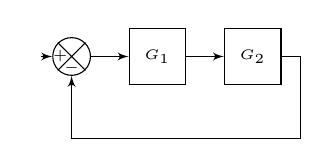
\begin{tikzpicture}\begin{tiny}\bXInput{A}\bXLoop[2]{A}{b/$G_1$,c/$G_2$}\end{tiny}\end{tikzpicture}&%
%      small 
%     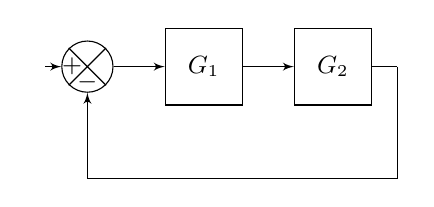
\begin{tikzpicture}\begin{small}\bXInput{A}\bXLoop[2]{A}{b/$G_1$,c/$G_2$}\end{small}\end{tikzpicture}\\ 
%      Normal
%     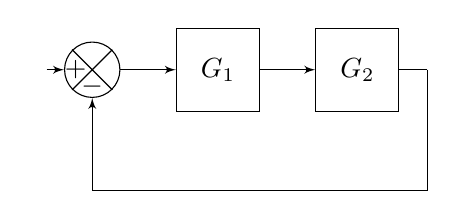
\begin{tikzpicture}\bXInput{A}\bXLoop[2]{A}{b/$G_1$,c/$G_2$}\end{tikzpicture}&%
%      Large
%     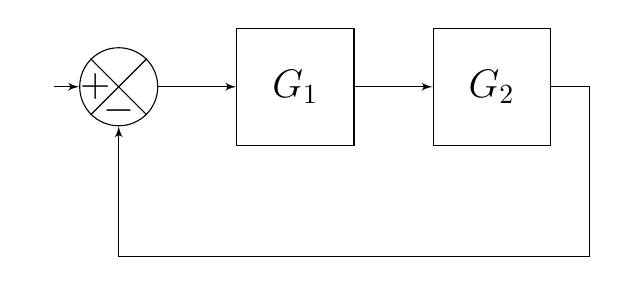
\begin{tikzpicture}\begin{Large}\bXInput{A}\bXLoop[2]{A}{b/$G_1$,c/$G_2$}\end{Large}\end{tikzpicture}
%  \end{tabular}
% \end{minipage}
% 
% \vspace{1em}
% \begin{minipage}{\textwidth}\vrbfnt
% \begin{verbatim}
% \begin{tabular}{p{.4\textwidth}p{.4\textwidth}}
%      tiny\hspace{1in} 
%     \begin{tikzpicture}\begin{tiny}\bXInput{A}\bXLoop[2]{A}{b/$G_1$,c/$G_2$}
%         \end{tiny}\end{tikzpicture}&%
%      small 
%     \begin{tikzpicture}\begin{small}\bXInput{A}\bXLoop[2]{A}{b/$G_1$,c/$G_2$}
%         \end{small}\end{tikzpicture}\\ 
%      Normal
%     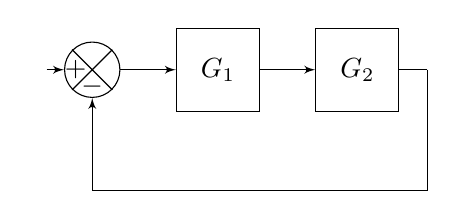
\begin{tikzpicture}\bXInput{A}\bXLoop[2]{A}{b/$G_1$,c/$G_2$}\end{tikzpicture}&%
%      Large
%     \begin{tikzpicture}\begin{Large}\bXInput{A}\bXLoop[2]{A}{b/$G_1$,c/$G_2$}
%         \end{Large}\end{tikzpicture}
%  \end{tabular}
% \end{verbatim}
% \end{minipage}
% \caption{A Scaling Example and Code}\label{fig:scaling}
% \end{figure}
%
% \section{Tips}
% \begin{itemize}
%  	\item If you want to work in the opposite direction than the normal one, use a negative \meta{distance}.  This can be useful when working with returns or branches.
% \item If you want text under a link, you can use |\bXLinkName| macro with a negative \meta{distance} and a \meta{Previous Node} of the form |D-E|.  
% 	\item It is always a good idea to draw the block diagram by hand first.  Then your code for this package, simple though it is, will be neater and easier to read because you can create the diagram in order.
% 	\item When something really special is needed, do not forget that you may use \stikz\ commands directly in your |tikzpicture| environment.  This is how I place the little filled-in blocks with the node names in Fig. \ref{fig:helps}.
%  \end{itemize}
% 
% \StopEventually{\PrintChanges\PrintIndex}
%
% \section{Implementation}
% Here is the listing of the source code for the package.  Most things here are as similar to the \textsf{schemabloc} package as I could make them.  These macros group sets of \stikz\ commands together to utilize the power of \stikz\ but allowing the user to not have to dig into \textsf{pgf/tikz}.
%
% Normal beginning package commands to provide for making sure the package works correctly.
%    \begin{macrocode}
\typeout{* }
\typeout{bloX: Just an English translation of schemabloc package.}
\typeout{bloX Copyright (C) 2014  Ben Reish}
\typeout{* }
\typeout{This program comes with ABSOLUTELY NO WARRANTY.}
\typeout{This is free software, and you are welcome to redistribute it}
\typeout{under certain conditions.}
\typeout{* }
%    \end{macrocode}
%
% The package has external dependencies beyond the base installation.  I am sorry.  
%    \begin{macrocode}
\RequirePackage{ifthen}
\RequirePackage{tikz}
\RequirePackage{pgffor}
\usetikzlibrary{shapes,arrows}
%    \end{macrocode}
% 
% Using the \stikz\ commands, initialize the styles for links, blocks, potatoes, and summing junctions.  
%    \begin{macrocode}
\tikzstyle{bXLineStyle}=[->,>=latex',]
\tikzstyle{bXStyleBloc}=[draw, rectangle,]
\tikzstyle{bXStyleBlocPotato}=[]
\tikzstyle{bXStyleSum}=[draw, circle,]%style Sum CC
\tikzstyle{bXLabelStyle}=[]
%    \end{macrocode}
% \begin{macro}{\bXDefaultLineStyle}\begin{macro}{\bXLineStyle}
% |\bXDefaultLineStyle| is used to re-establish the default line style once it has been changed by the below commands.  It defines a solid line with a \LaTeX\ style arrow tip.  
% To change the default line style, |\bXLineStyle| takes one argument which is added to the default line description by \stikz.
%    \begin{macrocode}
\newcommand{\bXDefaultLineStyle}{
\tikzstyle{bXLineStyle}=[->,>=latex']
}
\newcommand{\bXLineStyle}[1]{
\tikzstyle{bXLineStyle}+=[#1]
}
%    \end{macrocode}
% \end{macro}\end{macro}
% \begin{macro}{\bXStyleBloc}% \begin{macro}{\bXStyleBlocDefault}
% To re-establish the block style, use |\bXStyleBlocDefault|.  To change the default, the |\bXStyleBloc| command will take an argument and add it to the current block style definition.
%    \begin{macrocode}
\newcommand{\bXStyleBloc}[1]{
\tikzstyle{bXStyleBloc}+=[#1]
}
\newcommand{\bXStyleBlocDefault}{
\tikzstyle{bXStyleBloc}=[draw, rectangle,]
}
%    \end{macrocode}
% \end{macro}
% \end{macro}
% \begin{macro}{\bXStylePotato}% \begin{macro}{\bXStylePotatoDefault}
% To re-establish the potato block style, use |\bXStylePotatoDefault|.  To change the default, the |\bXStylePotato| command will take an argument and add it to the current block style definition. \changes{v2.3}{2014/08/14}{Added the style commands for the potato which were missing.}
%    \begin{macrocode}
\newcommand{\bXStylePotato}[1]{
\tikzstyle{bXStyleBlocPotato}+=[#1]
}
\newcommand{\bXStylePotatoDefault}{
\tikzstyle{bXStyleBlocPotato}=[draw, cloud, cloud puffs=5,]
}
%    \end{macrocode}
% \end{macro}
% \end{macro}
% \begin{macro}{\bXStyleSum}\begin{macro}{\bXStyleSumDefault}
% To re-establish the block style, use |\bXStyleSumDefault|.  To change the default, the |\bXStyleSum| command will take an argument and add it to the current sum style definition.
%    \begin{macrocode}
\newcommand{\bXStyleSum}[1]{
\tikzstyle{bXStyleSum}+=[#1]
}
\newcommand{\bXStyleSumDefault}{
\tikzstyle{bXStyleSum}=[draw, circle,]
}
%    \end{macrocode}
% \end{macro}\end{macro}
% \begin{macro}{\bXLabelStyle}\begin{macro}{\bXLabelStyleDefault}
% To re-establish the label style, use |\bXLabelStyleDefault|.  To change the default, the |\bXLabelStyle| command will take an argument and add it to the current label style definition.  This is used with the |\bXInput| and the |\bXLinkName| macros to customize the text. 
% \changes{v2.4}{2014/08/17}{Added a label style and default command to the bXInput and bXLinkName macros to allow customization of the font these two display.}
%    \begin{macrocode}
\newcommand{\bXLabelStyle}[1]{
\tikzstyle{bXLabelStyle}+=[#1]
}
\newcommand{\bXLabelStyleDefault}{
\tikzstyle{bXLabelStyle}=[font=\normalfont,]
}
%    \end{macrocode}
% \end{macro}\end{macro}
% \begin{macro}{\bXInput}
% I redefined the beginning command of the block diagram to take an optional argument and place it as a label above the node.  This required splitting the |\bXInput| command into three commands.  The user level command is |\bXInput| which looks to see if the next character is a `|[|'.  If so, it calls |\bXInputi|, else it calls |\bXInputii|.  If the optional argument is used, the |\bXInputi| command takes the list of arguments and processes them. The |\bXBranchx| is called to create the extra node labels for connecting links. \changes{v2.4}{2014/08/18}{Added usage bXLabelStyle}
%    \begin{macrocode}
\newcommand{\bXInput}{%
    \@ifnextchar[{\@bXInputi}{\@bXInputii}
}
\newcommand{\@bXInputi}[2][]{%
    \node [coordinate,name=#2,bXLabelStyle] {#1};
    \bXBranchx[0]{#2}{#2};
    \draw (0,0) node [anchor=east,name=#2label,] {#1};
}
\newcommand{\@bXInputii}[1]{%
    \node [coordinate,name=#1] { };
    \bXBranchx[0]{#1}{#1};
}
%    \end{macrocode}
% \end{macro}
%
% \begin{macro}{\bXOutput}
% To end the block diagram with an arrow pointing to the right, place a node at the right of the previous node to which a link can connect.
%    \begin{macrocode}
\newcommand{\bXOutput}[3][2]{
    \node [coordinate, right of=#3right, 
    node distance=#1em, minimum size=0em,right] (#2) {};
}
%    \end{macrocode}
% \end{macro}
%
% \begin{macro}{\bXBloc}\begin{macro}{\bXBlocr}\begin{macro}{\bXBlocL}\begin{macro}{\bXBlocrL}
% These commands create the paths which make the normal blocks, the return blocks, the normal block with link, and the return block with link.  The big difference between normal blocks and return blocks is that the orientation is switched. Instead of being placed to the right of the previous node, the return blocks are placed to the left.  
%    \begin{macrocode}
\newcommand{\bXBloc}[4][2]{
\node [draw, rectangle, 
    minimum height=3em, minimum width=3em, right of = #4right,
node distance=#1em,bXStyleBloc,right] (#2) {#3};
\node (#2right) at (#2.east){};
\node (Blocrightend) at (#2.east){};
}
\newcommand{\bXBlocr}[4][2]{
\node [ 
    minimum height=3em, minimum width=3em, left of = #4left, 
node distance=#1em, bXStyleBloc,left] (#2) {#3};
\node (#2left) at (#2.west){};
}
\newcommand{\bXBlocL}[4][2]{
\node [draw, rectangle, 
    minimum height=3em, minimum width=3em, 
    right of = #4right,node distance=#1em,bXStyleBloc,right] (#2) {#3};
\node (#2right) at (#2.east){};
\node (Blocrightend) at (#2.east){};
 \draw [bXLineStyle,auto] (#4) -- node[name=#4-#2] {} (#2);
}
\newcommand{\bXBlocrL}[4][2]{
\node [draw, rectangle, 
    minimum height=3em, minimum width=3em, left of = #4left, 
node distance=#1em, bXStyleBloc,left] (#2) {#3};
\node (#2left) at (#2.west){};
\node (Blocleftend) at (#2.west){};
 \draw [bXLineStyle,auto] (#4) -- node[name=#4-#2] {} (#2);
}

%    \end{macrocode}
% \end{macro}\end{macro}\end{macro}\end{macro}
% \begin{macro}{\bXBlocPotato}
% This command gives the user an option for a nondescript object by using \stikz's built in |cloud| keyword.  
%    \begin{macrocode}
\newcommand{\bXBlocPotato}[4][2]{
\node [draw, cloud, cloud puffs=5, draw, 
    minimum height=3em, minimum width=5em, right of = #4right,
node distance=#1em,bXStyleBlocPotato,right] (#2) {#3};
\node (#2right) at (#2.east){};
}
%    \end{macrocode}
% \end{macro}
%
% \begin{macro}{\bXOnlyOneBloc}
% This macro creates an entire single block, block diagram by itself.  It adds an input, a block, an output, and two links with the four arguments being the labels for everything.
%    \begin{macrocode}
\newcommand{\bXonlyOneBloc}[4][1.5]{
\bXInput{E1}
\bXBloc[#1]{B1}{#3}{E1}
\bXOutput[#1]{S1}{B1}
\bXLink{E1}{B1}{#2}
\bXLink{B1}{S1}{#4}
}
%    \end{macrocode}
% \end{macro}
%
% \begin{macro}{\bXLink}\begin{macro}{\bXLinkxy}\begin{macro}{\bXLinkyx}
% These macros tell \stikz\ where to place links, between which blocks.  The normal macro is |\bXLink| which takes 3 arguments.  It draws straight lines between the right edge of the previous node and the left edge of the next node.  It names the link \meta{Previous Node}-\meta{Next Node}. This allows the selection of the middle of the link between to blocks for the having a return link drawn from.  This macro will draw diagonal lines between nodes on different branches of a diagram.  To maintain square corners, use the |\bXLinkxy| to go first horizontally, then vertically; or use |\bXLinkyx| to go first vertically and then horizontally.    
%    \begin{macrocode}
\newcommand{\bXLink}[3][]{
 \draw [bXLineStyle,auto] (#2) -- node[name=#2-#3] {#1} (#3);
}
\newcommand{\bXLinkyx}[2]{
\draw [bXLineStyle] (#1.south)  |-   (#2)  ;
}
\newcommand{\bXLinkxy}[3][]{
\draw [bXLineStyle] (#2)  -|  
    node[name=#2-#3,near end,right] {#1} (#3) ;
}
%    \end{macrocode}
% \begin{macro}{\bXReturn}
%   This macro creates two nodes, one directly below the second argument and one directly below the third argument.  Then it draws straight lines to connect them.  
%    \begin{macrocode}
\newcommand{\bXReturn}[4][4]{
\node [below of=#2, node distance=#1em,
    minimum size=0em](return#2) {};
\draw [bXLineStyle] (#2.south)--(return#2.south)  
-|   node[name=#2-#3,near end,right] {#4} (#3) ;
}
%    \end{macrocode}
% \begin{macro}{\bXLinkName}
% This macro adds a label to the output of a diagram at the end like the optional argument does on the input of the diagram.  
%    \begin{macrocode}
\newcommand{\bXLinkName}[3][0.4]{
\node[above of=#2, node distance=#1em, bXLabelStyle] (#2name) at (#2) {#3};
}
%    \end{macrocode}
% \end{macro}\end{macro}\end{macro}\end{macro}\end{macro}
%
% \begin{macro}{\bXCompSum}
% |\bXCompSum| is broken into three macros to be able to accommodate the starred version.  They all are user level commands so they can be called directly.  Generally, though, use |\bXCompSum| or |\bXCompSum*|.  |\bXCompSum| will check if the next character is a |*|. If so, it will call |\bXCompSumNorm|. Otherwise, it calls |\bXCompSumOnly|.   |\bXCompSumOnly| places the `X' in the circle and creates four nodes for the labels of the last four arguments inside the circle.  The other command places the last four arguments outside the circle. 
%
% \changes{v2.4}{2014/08/14}{Converted bXCompSumNorm and bXCompSumOnly to private functions.} Update: I converted |\bXCompSumNorm| and |\bXCompSumOnly|  to private functions.  Now they have |@|'s in them.
%    \begin{macrocode}
\newcommand*{\bXCompSum}{\@ifstar\bX@CompSumNorm\bX@CompSumOnly}
\newcommand{\bX@CompSumOnly}[7][4]{
    \node [draw, circle,minimum size=2em, 
	right of=#3,node distance=#1em] (#2) {};
    \node [draw, cross out,minimum size=1.414em,
	right of=#3,node distance=#1em] {};
    \node [above of=#2,node distance=0.6em] {$#4$};
    \node [below of=#2,node distance=0.6em] {$#5$};
    \node [left of=#2,node distance=0.6em] {$#6$};
    \node [right of=#2,node distance=0.6em] {$#7$};
\node (#2right) at (#2.east){};
\node (#2left) at (#2.west){};
}
\newcommand{\bX@CompSumNorm}[7][4]{
    \node [draw, circle,minimum size=1.5em,
	right of=#3,node distance=#1em,
	label=85:$#4$,label=-85:$#5$,label=175:$#6$,
	label=5:$#7$,bXStyleSum] (#2) {};
\node (#2right) at (#2.east){};
\node (#2left) at (#2.west){};
}
%    \end{macrocode}
% \end{macro}
%
% \begin{macro}{\bXComp}
% In an effort to reduce the keystrokes needed to produce a comparator, |\bXComp| is offered.  It is broken into three macros to take care of whether or not the user wants an `X'.  These macros just hardcode some inputs to the |\bXCompSum| macro.  
% \changes{v2.4}{2014/08/14}{Converted bXCompNorm and bXCompOnly to private functions.}
%    \begin{macrocode}
\newcommand*{\bXComp}{\@ifstar\bX@CompNorm\bX@CompOnly}
\newcommand{\bX@CompOnly}[3][4]{
\bXCompSum[#1]{#2}{#3}{}{-}{+}{}
}
\newcommand{\bX@CompNorm}[3][4]{
\bXCompSum*[#1]{#2}{#3}{}{-}{+}{}
}
%    \end{macrocode}
% \end{macro}
%
% \begin{macro}{\bXCompa}
% Again, in an effort to reduce keystrokes, a macro is offered to make a comparator whose negative input is from above.  It, too, is split into three macros to handle the starred version.  
% \changes{v2.4}{2014/08/14}{Converted bXCompaNorm and bXCompaOnly to private functions.}
%    \begin{macrocode}
\newcommand*{\bXCompa}{\@ifstar\bX@CompaNorm\bX@CompaOnly}
\newcommand{\bX@CompaOnly}[3][4]{
\bXCompSum[#1]{#2}{#3}{-}{}{+}{}
}
\newcommand{\bX@CompaNorm}[3][4]{
\bXCompSum*[#1]{#2}{#3}{-}{}{+}{}
}
%    \end{macrocode}
% \end{macro}
%
% \begin{macro}{\bXSuma}
% To meet the same need as that of |\bXCompa|, but with a summing junction, |\bXSuma| is offered.
% \changes{v2.4}{2014/08/14}{Converted bXSumaNorm and bXSumaOnly to private functions.}
%    \begin{macrocode}
\newcommand*{\bXSuma}{\@ifstar\bX@SumaNorm\bX@SumaOnly}
\newcommand{\bX@SumaOnly}[3][4]{
\bXCompSum[#1]{#2}{#3}{+}{}{+}{}
}
\newcommand{\bX@SumaNorm}[3][4]{
\bXCompSum*[#1]{#2}{#3}{+}{}{+}{}
}
%    \end{macrocode}
% \end{macro}
%
% \begin{macro}{\bXSumb}
% To meet the same need as that of |\bXComp|, but with a summing junction, |\bXSumb| is offered.
% \changes{v2.4}{2014/08/14}{Converted bXSumbNorm and bXSumbOnly to private functions.}
%    \begin{macrocode}
\newcommand*{\bXSumb}{\@ifstar\bX@SumbNorm\bX@SumbOnly}
\newcommand{\bX@SumbOnly}[3][4]{
\bXCompSum[#1]{#2}{#3}{}{+}{+}{}
}
\newcommand{\bX@SumbNorm}[3][4]{
\bXCompSum*[#1]{#2}{#3}{}{+}{+}{}
}
%    \end{macrocode}
% \end{macro}
%
% \begin{macro}{\bXSum}
% I think this macro is for printing out an empty comparator or summing junction with few keystrokes.  I think it is redundant, but here it is.  
%    \begin{macrocode}
\newcommand{\bXSum}[6][4]{
    \node [draw, circle,minimum size=1.5em, 
	right of=#3,node distance=#1em,
	label=175:$#4$,label=-85:$#5$,
	label=85:$#6$,bXStyleSum] (#2) {};
\node (#2right) at (#2.east){};
\node (#2left) at (#2.west){};
}
%    \end{macrocode}
% \end{macro}
% \begin{macro}{\bXBranchy}\begin{macro}{\bXNodeShifty}
% The |\bXBranchy| macro is used to create a node vertically displaced from the third argument by the first argument.  This allows for multiple inputs and outputs in a block diagram.  It creates the node names right and left for other macros to use.  The |\bXNodeShifty| macro is retained for version compatability.  
%    \begin{macrocode}
\newcommand{\bXBranchy}[3][5]{
\node [below of=#2, node distance=#1em, minimum size=0em](#3) {};
\node (#3right) at (#3){};
\node (#3left) at (#3){};
}
\newcommand{\bXNodeShifty}[3][5]{
    \bXBranchy[#1]{#2}{#3}
}
%    \end{macrocode}
% \end{macro}\end{macro}
% \begin{macro}{\bXBranchx}\begin{macro}{\bXNodeShiftx}
% The |\bXBranchx| macro is used to create a node horizontally displaced from the third argument by the first argument.  It creates the node names right and left for other macros to use.  The |\bXNodeShiftx| macro is retained for version compatability.  
%    \begin{macrocode}
\newcommand{\bXBranchx}[3][5]{
\node [right of=#2, node distance=#1em, minimum size=0em](#3) {};
\node (#3right) at (#3){};
\node (#3left) at (#3){};
}
\newcommand{\bXNodeShiftx}[3][5]{
    \bXBranchx[#1]{#2}{#3}
}
%    \end{macrocode}
% \end{macro}\end{macro}
% \begin{macro}{\bXChain}
% A chain is a set of blocks connected to each other created from a list.  This function leans heavily on the \stikz\ |foreach| command.  There are a couple of special versions of this command which were previously (in \textsf{schemabloc}) used together unsuccessfully. I don't think \stikz\ allows the combination of its versions of the |foreach| command.  I simplified the use to be a selection from a list of comma-separated values of the form: a/b,c/d,\ldots which was useful to me.  I then used a global let statement to redefine what |\lastx| was each iteration.  This seems to work. The |\typeout| is for debugging.  I like the lists so I left it un-commented.  
% \changes{v2.0}{2014/08/01}{Simplified the foreach statement from tikz and applied a global let statement}
%    \begin{macrocode}
\newcommand{\bXChain}[3][4]{
    \def\lastx{#2}%
    \foreach \x / \y  in {#3}%
    {\bXBlocL[#1]{\x}{\y}{\lastx} %
    \typeout{\x, \y, \lastx}%
    \global\let\lastx\x}
}
%    \end{macrocode}
% \end{macro}
%
% \begin{macro}{\bXChainReturn}
% This macro has the same machinations that the previous one does, but is to be used on the return side, so the block command is swapped out with |\bXBlocrL|.  Otherwise, it works just as the |\bXChain| macro does.  
%    \begin{macrocode}
\newcommand{\bXChainReturn}[3][4]{
    \def\lastx{#2}%
    \foreach \x / \y  in {#3}%
    {\bXBlocrL[#1]{\x}{\y}{\lastx} %
    \typeout{\x, \y, \lastx}%
    \global\let\lastx\x}
}
%    \end{macrocode}
% \end{macro}
%
% \begin{macro}{\bXOnlyLoop}
% This command is supposed to create a block diagram for you, but it errors out so I have removed it from this version of the \blox\ package.  \stikz\ can not find a node that it is looking for and I haven't figured that one out yet.  
% \changes{v2.2}{2014/08/13}{Removed the bXOnlyLoop macro and bXLoopReturn macro for further study.}
%    \begin{macrocode}
% \newcommand{\bXOnlyLoop}[4][4]{
% \bXComp[#1]{Comp#2}{#2}\bXLink{#2}{Comp#2}
% \bXChain[#1]{Comp#2}{#3}
% \bXOutput[#1]{#4}{BlocdeFin}
% \draw [bXLineStyle,auto] (Blocrightend.base) -- 
%   node[name=FindeChain-#4] {} (#4);
% \bXReturn{FindeChain-#4}{Comp#2}{}
% }
%    \end{macrocode}
% \end{macro}
%
% \begin{macro}{\bXLoop}
% This macro is designed to make a loop diagram from a list of values. You make an input and then hand this macro a \meta{distance}, the name of your input, and a list like: |a/$G_1$,b/$G_2$|.  It just draws a line from the end of the list of block back to the comparator.  
%    \begin{macrocode}
\newcommand{\bXLoop}[3][4]{
\bXComp[#1]{Comp#2}{#2}\bXLink{#2}{Comp#2}
\bXChain[#1]{Comp#2}{#3}
\draw [bXLineStyle,auto,-] (Blocrightend.base) --++ 
    (1em,0)coordinate[name=EndofChain];
\bXReturn{EndofChain}{Comp#2}{}
}
%    \end{macrocode}
% \end{macro}
%
% \begin{macro}{\bXLoopReturn}
% This is the same idea as the previous macro, but adds a second list argument which allows for a set of blocks to be set on the return loop as well.  It, too, does not work properly, so I have commented it out of this version.  
%    \begin{macrocode}
% \newcommand{\bXLoopReturn}[4][4]{
% \bXComp[#1]{Comp#2}{#2}\bXLink{#2}{Comp#2}
% \bXChain[#1]{Comp#2}{#3}
% \draw [bXLineStyle,auto,-] (Blocrightend.base) --++
%     (1em,0)coordinate[name=FindeChain];
% \bXBranchy[5]{FindeChain}{bXDebutReturn}
% \bXChainReturn[#1]{bXDebutReturn}{#4}
% \draw [bXLineStyle,-] (FindeChain)  |-   (bXDebutReturn.west)  ;
% \draw [bXLineStyle] (Blocleftend.base)  -| 
% node[name=bXNomReturn,near end,right] {} (Comp#2) ;
% }
%    \end{macrocode}
% \end{macro}
% \Finale
\endinput